\documentclass[twoside]{book}

% Packages required by doxygen
\usepackage{fixltx2e}
\usepackage{calc}
\usepackage{doxygen}
\usepackage[export]{adjustbox} % also loads graphicx
\usepackage{graphicx}
\usepackage[utf8]{inputenc}
\usepackage{makeidx}
\usepackage{multicol}
\usepackage{multirow}
\PassOptionsToPackage{warn}{textcomp}
\usepackage{textcomp}
\usepackage[nointegrals]{wasysym}
\usepackage[table]{xcolor}

% NLS support packages
\usepackage[spanish]{babel}
% Font selection
\usepackage[T1]{fontenc}
\usepackage[scaled=.90]{helvet}
\usepackage{courier}
\usepackage{amssymb}
\usepackage{sectsty}
\renewcommand{\familydefault}{\sfdefault}
\allsectionsfont{%
  \fontseries{bc}\selectfont%
  \color{darkgray}%
}
\renewcommand{\DoxyLabelFont}{%
  \fontseries{bc}\selectfont%
  \color{darkgray}%
}
\newcommand{\+}{\discretionary{\mbox{\scriptsize$\hookleftarrow$}}{}{}}

% Page & text layout
\usepackage{geometry}
\geometry{%
  a4paper,%
  top=2.5cm,%
  bottom=2.5cm,%
  left=2.5cm,%
  right=2.5cm%
}
\tolerance=750
\hfuzz=15pt
\hbadness=750
\setlength{\emergencystretch}{15pt}
\setlength{\parindent}{0cm}
\setlength{\parskip}{3ex plus 2ex minus 2ex}
\makeatletter
\renewcommand{\paragraph}{%
  \@startsection{paragraph}{4}{0ex}{-1.0ex}{1.0ex}{%
    \normalfont\normalsize\bfseries\SS@parafont%
  }%
}
\renewcommand{\subparagraph}{%
  \@startsection{subparagraph}{5}{0ex}{-1.0ex}{1.0ex}{%
    \normalfont\normalsize\bfseries\SS@subparafont%
  }%
}
\makeatother

% Headers & footers
\usepackage{fancyhdr}
\pagestyle{fancyplain}
\fancyhead[LE]{\fancyplain{}{\bfseries\thepage}}
\fancyhead[CE]{\fancyplain{}{}}
\fancyhead[RE]{\fancyplain{}{\bfseries\leftmark}}
\fancyhead[LO]{\fancyplain{}{\bfseries\rightmark}}
\fancyhead[CO]{\fancyplain{}{}}
\fancyhead[RO]{\fancyplain{}{\bfseries\thepage}}
\fancyfoot[LE]{\fancyplain{}{}}
\fancyfoot[CE]{\fancyplain{}{}}
\fancyfoot[RE]{\fancyplain{}{\bfseries\scriptsize Generado por Doxygen }}
\fancyfoot[LO]{\fancyplain{}{\bfseries\scriptsize Generado por Doxygen }}
\fancyfoot[CO]{\fancyplain{}{}}
\fancyfoot[RO]{\fancyplain{}{}}
\renewcommand{\footrulewidth}{0.4pt}
\renewcommand{\chaptermark}[1]{%
  \markboth{#1}{}%
}
\renewcommand{\sectionmark}[1]{%
  \markright{\thesection\ #1}%
}

% Indices & bibliography
\usepackage{natbib}
\usepackage[titles]{tocloft}
\setcounter{tocdepth}{3}
\setcounter{secnumdepth}{5}
\makeindex

% Hyperlinks (required, but should be loaded last)
\usepackage{ifpdf}
\ifpdf
  \usepackage[pdftex,pagebackref=true]{hyperref}
\else
  \usepackage[ps2pdf,pagebackref=true]{hyperref}
\fi
\hypersetup{%
  colorlinks=true,%
  linkcolor=blue,%
  citecolor=blue,%
  unicode%
}

% Custom commands
\newcommand{\clearemptydoublepage}{%
  \newpage{\pagestyle{empty}\cleardoublepage}%
}

\usepackage{caption}
\captionsetup{labelsep=space,justification=centering,font={bf},singlelinecheck=off,skip=4pt,position=top}

%===== C O N T E N T S =====

\begin{document}

% Titlepage & ToC
\hypersetup{pageanchor=false,
             bookmarksnumbered=true,
             pdfencoding=unicode
            }
\pagenumbering{alph}
\begin{titlepage}
\vspace*{7cm}
\begin{center}%
{\Large Music.\+IO }\\
\vspace*{1cm}
{\large Generado por Doxygen 1.8.13}\\
\end{center}
\end{titlepage}
\clearemptydoublepage
\pagenumbering{roman}
\tableofcontents
\clearemptydoublepage
\pagenumbering{arabic}
\hypersetup{pageanchor=true}

%--- Begin generated contents ---
\chapter{Indice jerárquico}
\section{Jerarquía de la clase}
Esta lista de herencias esta ordenada aproximadamente por orden alfabético\+:\begin{DoxyCompactList}
\item App\+Compat\+Edit\+Text\begin{DoxyCompactList}
\item \contentsline{section}{com.\+example.\+mediaio.\+mediaio.\+Formularios.\+Edit\+Text\+Comun}{\pageref{classcom_1_1example_1_1mediaio_1_1mediaio_1_1_formularios_1_1_edit_text_comun}}{}
\item \contentsline{section}{com.\+example.\+mediaio.\+mediaio.\+Formularios.\+Edit\+Text\+Email}{\pageref{classcom_1_1example_1_1mediaio_1_1mediaio_1_1_formularios_1_1_edit_text_email}}{}
\item \contentsline{section}{com.\+example.\+mediaio.\+mediaio.\+Formularios.\+Edit\+Text\+Fecha}{\pageref{classcom_1_1example_1_1mediaio_1_1mediaio_1_1_formularios_1_1_edit_text_fecha}}{}
\item \contentsline{section}{com.\+example.\+mediaio.\+mediaio.\+Formularios.\+Edit\+Text\+Password}{\pageref{classcom_1_1example_1_1mediaio_1_1mediaio_1_1_formularios_1_1_edit_text_password}}{}
\end{DoxyCompactList}
\item Exception\begin{DoxyCompactList}
\item \contentsline{section}{com.\+example.\+mediaio.\+mediaio.\+Excepciones.\+Input\+Erronea}{\pageref{classcom_1_1example_1_1mediaio_1_1mediaio_1_1_excepciones_1_1_input_erronea}}{}
\end{DoxyCompactList}
\item \contentsline{section}{com.\+example.\+mediaio.\+mediaio.\+modelo.\+Interfaz\+Rest}{\pageref{classcom_1_1example_1_1mediaio_1_1mediaio_1_1modelo_1_1_interfaz_rest}}{}
\begin{DoxyCompactList}
\item \contentsline{section}{com.\+example.\+mediaio.\+mediaio.\+modelo.\+Shared\+Server}{\pageref{classcom_1_1example_1_1mediaio_1_1mediaio_1_1modelo_1_1_shared_server}}{}
\end{DoxyCompactList}
\item \contentsline{section}{com.\+example.\+mediaio.\+mediaio.\+modelo.\+J\+S\+O\+N\+Callback}{\pageref{classcom_1_1example_1_1mediaio_1_1mediaio_1_1modelo_1_1_j_s_o_n_callback}}{}
\begin{DoxyCompactList}
\item \contentsline{section}{com.\+example.\+mediaio.\+mediaio.\+Login\+First\+Activity.\+Verificar\+Email}{\pageref{classcom_1_1example_1_1mediaio_1_1mediaio_1_1_login_first_activity_1_1_verificar_email}}{}
\end{DoxyCompactList}
\item \contentsline{section}{com.\+example.\+mediaio.\+mediaio.\+modelo.\+Mensaje\+Firebase}{\pageref{classcom_1_1example_1_1mediaio_1_1mediaio_1_1modelo_1_1_mensaje_firebase}}{}
\item App\+Compat\+Activity\begin{DoxyCompactList}
\item \contentsline{section}{com.\+example.\+mediaio.\+mediaio.\+Actividades.\+Actividad\+Principal}{\pageref{classcom_1_1example_1_1mediaio_1_1mediaio_1_1_actividades_1_1_actividad_principal}}{}
\begin{DoxyCompactList}
\item \contentsline{section}{com.\+example.\+mediaio.\+mediaio.\+Media\+I\+O\+Main}{\pageref{classcom_1_1example_1_1mediaio_1_1mediaio_1_1_media_i_o_main}}{}
\item \contentsline{section}{com.\+example.\+mediaio.\+mediaio.\+Media\+I\+O\+Perfil}{\pageref{classcom_1_1example_1_1mediaio_1_1mediaio_1_1_media_i_o_perfil}}{}
\item \contentsline{section}{com.\+example.\+mediaio.\+mediaio.\+Media\+I\+O\+Play}{\pageref{classcom_1_1example_1_1mediaio_1_1mediaio_1_1_media_i_o_play}}{}
\end{DoxyCompactList}
\item \contentsline{section}{com.\+example.\+mediaio.\+mediaio.\+Login\+First\+Activity}{\pageref{classcom_1_1example_1_1mediaio_1_1mediaio_1_1_login_first_activity}}{}
\item \contentsline{section}{com.\+example.\+mediaio.\+mediaio.\+Login\+Second\+Activity}{\pageref{classcom_1_1example_1_1mediaio_1_1mediaio_1_1_login_second_activity}}{}
\item \contentsline{section}{com.\+example.\+mediaio.\+mediaio.\+Main\+Activity}{\pageref{classcom_1_1example_1_1mediaio_1_1mediaio_1_1_main_activity}}{}
\item \contentsline{section}{com.\+example.\+mediaio.\+mediaio.\+Media\+I\+O\+Chat}{\pageref{classcom_1_1example_1_1mediaio_1_1mediaio_1_1_media_i_o_chat}}{}
\item \contentsline{section}{com.\+example.\+mediaio.\+mediaio.\+Media\+I\+O\+Registrar}{\pageref{classcom_1_1example_1_1mediaio_1_1mediaio_1_1_media_i_o_registrar}}{}
\end{DoxyCompactList}
\item Async\+Task\begin{DoxyCompactList}
\item \contentsline{section}{com.\+example.\+mediaio.\+mediaio.\+modelo.\+Reproductor}{\pageref{classcom_1_1example_1_1mediaio_1_1mediaio_1_1modelo_1_1_reproductor}}{}
\end{DoxyCompactList}
\item List\+Adapter\begin{DoxyCompactList}
\item \contentsline{section}{com.\+example.\+mediaio.\+mediaio.\+modelo.\+Adapter\+Canciones}{\pageref{classcom_1_1example_1_1mediaio_1_1mediaio_1_1modelo_1_1_adapter_canciones}}{}
\end{DoxyCompactList}
\end{DoxyCompactList}

\chapter{Índice de clases}
\section{Lista de clases}
Lista de las clases, estructuras, uniones e interfaces con una breve descripción\+:\begin{DoxyCompactList}
\item\contentsline{section}{\hyperlink{classcom_1_1example_1_1mediaio_1_1mediaio_1_1_actividades_1_1_actividad_principal}{com.\+example.\+mediaio.\+mediaio.\+Actividades.\+Actividad\+Principal} }{\pageref{classcom_1_1example_1_1mediaio_1_1mediaio_1_1_actividades_1_1_actividad_principal}}{}
\item\contentsline{section}{\hyperlink{classcom_1_1example_1_1mediaio_1_1mediaio_1_1modelo_1_1_adapter_canciones}{com.\+example.\+mediaio.\+mediaio.\+modelo.\+Adapter\+Canciones} }{\pageref{classcom_1_1example_1_1mediaio_1_1mediaio_1_1modelo_1_1_adapter_canciones}}{}
\item\contentsline{section}{\hyperlink{classcom_1_1example_1_1mediaio_1_1mediaio_1_1_formularios_1_1_edit_text_comun}{com.\+example.\+mediaio.\+mediaio.\+Formularios.\+Edit\+Text\+Comun} }{\pageref{classcom_1_1example_1_1mediaio_1_1mediaio_1_1_formularios_1_1_edit_text_comun}}{}
\item\contentsline{section}{\hyperlink{classcom_1_1example_1_1mediaio_1_1mediaio_1_1_formularios_1_1_edit_text_email}{com.\+example.\+mediaio.\+mediaio.\+Formularios.\+Edit\+Text\+Email} }{\pageref{classcom_1_1example_1_1mediaio_1_1mediaio_1_1_formularios_1_1_edit_text_email}}{}
\item\contentsline{section}{\hyperlink{classcom_1_1example_1_1mediaio_1_1mediaio_1_1_formularios_1_1_edit_text_fecha}{com.\+example.\+mediaio.\+mediaio.\+Formularios.\+Edit\+Text\+Fecha} }{\pageref{classcom_1_1example_1_1mediaio_1_1mediaio_1_1_formularios_1_1_edit_text_fecha}}{}
\item\contentsline{section}{\hyperlink{classcom_1_1example_1_1mediaio_1_1mediaio_1_1_formularios_1_1_edit_text_password}{com.\+example.\+mediaio.\+mediaio.\+Formularios.\+Edit\+Text\+Password} }{\pageref{classcom_1_1example_1_1mediaio_1_1mediaio_1_1_formularios_1_1_edit_text_password}}{}
\item\contentsline{section}{\hyperlink{classcom_1_1example_1_1mediaio_1_1mediaio_1_1_excepciones_1_1_input_erronea}{com.\+example.\+mediaio.\+mediaio.\+Excepciones.\+Input\+Erronea} }{\pageref{classcom_1_1example_1_1mediaio_1_1mediaio_1_1_excepciones_1_1_input_erronea}}{}
\item\contentsline{section}{\hyperlink{classcom_1_1example_1_1mediaio_1_1mediaio_1_1modelo_1_1_interfaz_rest}{com.\+example.\+mediaio.\+mediaio.\+modelo.\+Interfaz\+Rest} }{\pageref{classcom_1_1example_1_1mediaio_1_1mediaio_1_1modelo_1_1_interfaz_rest}}{}
\item\contentsline{section}{\hyperlink{classcom_1_1example_1_1mediaio_1_1mediaio_1_1modelo_1_1_j_s_o_n_callback}{com.\+example.\+mediaio.\+mediaio.\+modelo.\+J\+S\+O\+N\+Callback} }{\pageref{classcom_1_1example_1_1mediaio_1_1mediaio_1_1modelo_1_1_j_s_o_n_callback}}{}
\item\contentsline{section}{\hyperlink{classcom_1_1example_1_1mediaio_1_1mediaio_1_1_login_first_activity}{com.\+example.\+mediaio.\+mediaio.\+Login\+First\+Activity} }{\pageref{classcom_1_1example_1_1mediaio_1_1mediaio_1_1_login_first_activity}}{}
\item\contentsline{section}{\hyperlink{classcom_1_1example_1_1mediaio_1_1mediaio_1_1_login_second_activity}{com.\+example.\+mediaio.\+mediaio.\+Login\+Second\+Activity} }{\pageref{classcom_1_1example_1_1mediaio_1_1mediaio_1_1_login_second_activity}}{}
\item\contentsline{section}{\hyperlink{classcom_1_1example_1_1mediaio_1_1mediaio_1_1_main_activity}{com.\+example.\+mediaio.\+mediaio.\+Main\+Activity} }{\pageref{classcom_1_1example_1_1mediaio_1_1mediaio_1_1_main_activity}}{}
\item\contentsline{section}{\hyperlink{classcom_1_1example_1_1mediaio_1_1mediaio_1_1_media_i_o_chat}{com.\+example.\+mediaio.\+mediaio.\+Media\+I\+O\+Chat} }{\pageref{classcom_1_1example_1_1mediaio_1_1mediaio_1_1_media_i_o_chat}}{}
\item\contentsline{section}{\hyperlink{classcom_1_1example_1_1mediaio_1_1mediaio_1_1_media_i_o_main}{com.\+example.\+mediaio.\+mediaio.\+Media\+I\+O\+Main} }{\pageref{classcom_1_1example_1_1mediaio_1_1mediaio_1_1_media_i_o_main}}{}
\item\contentsline{section}{\hyperlink{classcom_1_1example_1_1mediaio_1_1mediaio_1_1_media_i_o_perfil}{com.\+example.\+mediaio.\+mediaio.\+Media\+I\+O\+Perfil} }{\pageref{classcom_1_1example_1_1mediaio_1_1mediaio_1_1_media_i_o_perfil}}{}
\item\contentsline{section}{\hyperlink{classcom_1_1example_1_1mediaio_1_1mediaio_1_1_media_i_o_play}{com.\+example.\+mediaio.\+mediaio.\+Media\+I\+O\+Play} }{\pageref{classcom_1_1example_1_1mediaio_1_1mediaio_1_1_media_i_o_play}}{}
\item\contentsline{section}{\hyperlink{classcom_1_1example_1_1mediaio_1_1mediaio_1_1_media_i_o_registrar}{com.\+example.\+mediaio.\+mediaio.\+Media\+I\+O\+Registrar} }{\pageref{classcom_1_1example_1_1mediaio_1_1mediaio_1_1_media_i_o_registrar}}{}
\item\contentsline{section}{\hyperlink{classcom_1_1example_1_1mediaio_1_1mediaio_1_1modelo_1_1_mensaje_firebase}{com.\+example.\+mediaio.\+mediaio.\+modelo.\+Mensaje\+Firebase} }{\pageref{classcom_1_1example_1_1mediaio_1_1mediaio_1_1modelo_1_1_mensaje_firebase}}{}
\item\contentsline{section}{\hyperlink{classcom_1_1example_1_1mediaio_1_1mediaio_1_1modelo_1_1_reproductor}{com.\+example.\+mediaio.\+mediaio.\+modelo.\+Reproductor} }{\pageref{classcom_1_1example_1_1mediaio_1_1mediaio_1_1modelo_1_1_reproductor}}{}
\item\contentsline{section}{\hyperlink{classcom_1_1example_1_1mediaio_1_1mediaio_1_1modelo_1_1_shared_server}{com.\+example.\+mediaio.\+mediaio.\+modelo.\+Shared\+Server} }{\pageref{classcom_1_1example_1_1mediaio_1_1mediaio_1_1modelo_1_1_shared_server}}{}
\item\contentsline{section}{\hyperlink{classcom_1_1example_1_1mediaio_1_1mediaio_1_1_login_first_activity_1_1_verificar_email}{com.\+example.\+mediaio.\+mediaio.\+Login\+First\+Activity.\+Verificar\+Email} }{\pageref{classcom_1_1example_1_1mediaio_1_1mediaio_1_1_login_first_activity_1_1_verificar_email}}{}
\end{DoxyCompactList}

\chapter{Documentación de las clases}
\hypertarget{classcom_1_1example_1_1mediaio_1_1mediaio_1_1_actividades_1_1_actividad_principal}{}\section{Referencia de la Clase com.\+example.\+mediaio.\+mediaio.\+Actividades.\+Actividad\+Principal}
\label{classcom_1_1example_1_1mediaio_1_1mediaio_1_1_actividades_1_1_actividad_principal}\index{com.\+example.\+mediaio.\+mediaio.\+Actividades.\+Actividad\+Principal@{com.\+example.\+mediaio.\+mediaio.\+Actividades.\+Actividad\+Principal}}
Diagrama de herencias de com.\+example.\+mediaio.\+mediaio.\+Actividades.\+Actividad\+Principal\begin{figure}[H]
\begin{center}
\leavevmode
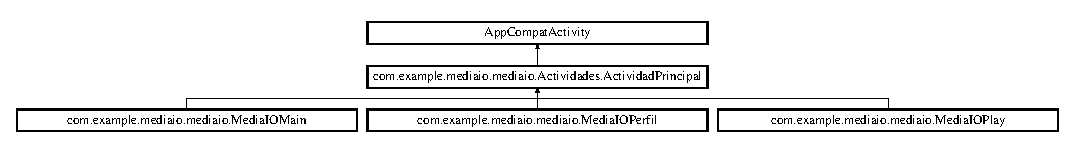
\includegraphics[height=1.538462cm]{classcom_1_1example_1_1mediaio_1_1mediaio_1_1_actividades_1_1_actividad_principal}
\end{center}
\end{figure}
\subsection*{Métodos públicos}
\begin{DoxyCompactItemize}
\item 
\mbox{\Hypertarget{classcom_1_1example_1_1mediaio_1_1mediaio_1_1_actividades_1_1_actividad_principal_a37f2b352b90ed62b99883932170b4d07}\label{classcom_1_1example_1_1mediaio_1_1mediaio_1_1_actividades_1_1_actividad_principal_a37f2b352b90ed62b99883932170b4d07}} 
boolean {\bfseries on\+Create\+Options\+Menu} (Menu menu)
\item 
\mbox{\Hypertarget{classcom_1_1example_1_1mediaio_1_1mediaio_1_1_actividades_1_1_actividad_principal_af757e79380d7a7caccf267274e1d6c9c}\label{classcom_1_1example_1_1mediaio_1_1mediaio_1_1_actividades_1_1_actividad_principal_af757e79380d7a7caccf267274e1d6c9c}} 
boolean {\bfseries on\+Options\+Item\+Selected} (Menu\+Item item)
\end{DoxyCompactItemize}
\subsection*{Métodos protegidos}
\begin{DoxyCompactItemize}
\item 
\mbox{\Hypertarget{classcom_1_1example_1_1mediaio_1_1mediaio_1_1_actividades_1_1_actividad_principal_ab7d3f06e9ac1e4eb36d33de3b6e0ec8c}\label{classcom_1_1example_1_1mediaio_1_1mediaio_1_1_actividades_1_1_actividad_principal_ab7d3f06e9ac1e4eb36d33de3b6e0ec8c}} 
void {\bfseries on\+Create} (Bundle saved\+Instance\+State)
\end{DoxyCompactItemize}


\subsection{Descripción detallada}
Created by Marcos on 15/04/2017. 

La documentación para esta clase fue generada a partir del siguiente fichero\+:\begin{DoxyCompactItemize}
\item 
E\+:/\+Users/\+Marcos/\+Android\+Studio\+Projects/\+Media.\+io/app/src/main/java/com/example/mediaio/mediaio/\+Actividades/Actividad\+Principal.\+java\end{DoxyCompactItemize}

\hypertarget{classcom_1_1example_1_1mediaio_1_1mediaio_1_1modelo_1_1_adapter_canciones}{}\section{Referencia de la Clase com.\+example.\+mediaio.\+mediaio.\+modelo.\+Adapter\+Canciones}
\label{classcom_1_1example_1_1mediaio_1_1mediaio_1_1modelo_1_1_adapter_canciones}\index{com.\+example.\+mediaio.\+mediaio.\+modelo.\+Adapter\+Canciones@{com.\+example.\+mediaio.\+mediaio.\+modelo.\+Adapter\+Canciones}}
Diagrama de herencias de com.\+example.\+mediaio.\+mediaio.\+modelo.\+Adapter\+Canciones\begin{figure}[H]
\begin{center}
\leavevmode
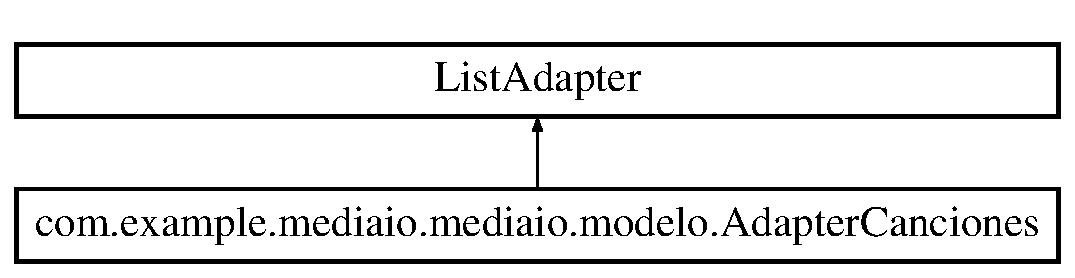
\includegraphics[height=2.000000cm]{classcom_1_1example_1_1mediaio_1_1mediaio_1_1modelo_1_1_adapter_canciones}
\end{center}
\end{figure}
\subsection*{Métodos públicos}
\begin{DoxyCompactItemize}
\item 
\mbox{\Hypertarget{classcom_1_1example_1_1mediaio_1_1mediaio_1_1modelo_1_1_adapter_canciones_a28ed701a3b734c5759bfc837b83f3b01}\label{classcom_1_1example_1_1mediaio_1_1mediaio_1_1modelo_1_1_adapter_canciones_a28ed701a3b734c5759bfc837b83f3b01}} 
{\bfseries Adapter\+Canciones} (\hyperlink{classcom_1_1example_1_1mediaio_1_1mediaio_1_1_actividades_1_1_actividad_principal}{Actividad\+Principal} contexto, List$<$ J\+S\+O\+N\+Object $>$ Lista\+Json)
\item 
\mbox{\Hypertarget{classcom_1_1example_1_1mediaio_1_1mediaio_1_1modelo_1_1_adapter_canciones_a96d95fa7357b3d9d7c8bb7ac2bdf8718}\label{classcom_1_1example_1_1mediaio_1_1mediaio_1_1modelo_1_1_adapter_canciones_a96d95fa7357b3d9d7c8bb7ac2bdf8718}} 
boolean {\bfseries are\+All\+Items\+Enabled} ()
\item 
\mbox{\Hypertarget{classcom_1_1example_1_1mediaio_1_1mediaio_1_1modelo_1_1_adapter_canciones_aa7bb61883df6d97f3a32fa6ef9e4e14e}\label{classcom_1_1example_1_1mediaio_1_1mediaio_1_1modelo_1_1_adapter_canciones_aa7bb61883df6d97f3a32fa6ef9e4e14e}} 
boolean {\bfseries is\+Enabled} (int position)
\item 
\mbox{\Hypertarget{classcom_1_1example_1_1mediaio_1_1mediaio_1_1modelo_1_1_adapter_canciones_a35495abacaae971fe3bea0f1b07ec0e5}\label{classcom_1_1example_1_1mediaio_1_1mediaio_1_1modelo_1_1_adapter_canciones_a35495abacaae971fe3bea0f1b07ec0e5}} 
void {\bfseries register\+Data\+Set\+Observer} (Data\+Set\+Observer observer)
\item 
\mbox{\Hypertarget{classcom_1_1example_1_1mediaio_1_1mediaio_1_1modelo_1_1_adapter_canciones_ac8c0877acc1913e5bea2aa11716de4d7}\label{classcom_1_1example_1_1mediaio_1_1mediaio_1_1modelo_1_1_adapter_canciones_ac8c0877acc1913e5bea2aa11716de4d7}} 
void {\bfseries unregister\+Data\+Set\+Observer} (Data\+Set\+Observer observer)
\item 
\mbox{\Hypertarget{classcom_1_1example_1_1mediaio_1_1mediaio_1_1modelo_1_1_adapter_canciones_ab01efefa426809c3a9500d4c98f9edbb}\label{classcom_1_1example_1_1mediaio_1_1mediaio_1_1modelo_1_1_adapter_canciones_ab01efefa426809c3a9500d4c98f9edbb}} 
int {\bfseries get\+Count} ()
\item 
\mbox{\Hypertarget{classcom_1_1example_1_1mediaio_1_1mediaio_1_1modelo_1_1_adapter_canciones_ac9526f08df06a74b4bf03ca997cc1281}\label{classcom_1_1example_1_1mediaio_1_1mediaio_1_1modelo_1_1_adapter_canciones_ac9526f08df06a74b4bf03ca997cc1281}} 
Object {\bfseries get\+Item} (int position)
\item 
\mbox{\Hypertarget{classcom_1_1example_1_1mediaio_1_1mediaio_1_1modelo_1_1_adapter_canciones_a56c15944afeae14894bd8298e990fc50}\label{classcom_1_1example_1_1mediaio_1_1mediaio_1_1modelo_1_1_adapter_canciones_a56c15944afeae14894bd8298e990fc50}} 
long {\bfseries get\+Item\+Id} (int position)
\item 
\mbox{\Hypertarget{classcom_1_1example_1_1mediaio_1_1mediaio_1_1modelo_1_1_adapter_canciones_a6fc28c896274cfc287e619834e26cc6b}\label{classcom_1_1example_1_1mediaio_1_1mediaio_1_1modelo_1_1_adapter_canciones_a6fc28c896274cfc287e619834e26cc6b}} 
boolean {\bfseries has\+Stable\+Ids} ()
\item 
\mbox{\Hypertarget{classcom_1_1example_1_1mediaio_1_1mediaio_1_1modelo_1_1_adapter_canciones_a958145ddb74c1070f005d0c29401f4aa}\label{classcom_1_1example_1_1mediaio_1_1mediaio_1_1modelo_1_1_adapter_canciones_a958145ddb74c1070f005d0c29401f4aa}} 
View {\bfseries get\+View} (int position, View convert\+View, View\+Group parent)
\item 
\mbox{\Hypertarget{classcom_1_1example_1_1mediaio_1_1mediaio_1_1modelo_1_1_adapter_canciones_a230d00b4dbea37cff1028a985165ab0b}\label{classcom_1_1example_1_1mediaio_1_1mediaio_1_1modelo_1_1_adapter_canciones_a230d00b4dbea37cff1028a985165ab0b}} 
int {\bfseries get\+Item\+View\+Type} (int position)
\item 
\mbox{\Hypertarget{classcom_1_1example_1_1mediaio_1_1mediaio_1_1modelo_1_1_adapter_canciones_a22277bc976749df7d497415056167957}\label{classcom_1_1example_1_1mediaio_1_1mediaio_1_1modelo_1_1_adapter_canciones_a22277bc976749df7d497415056167957}} 
int {\bfseries get\+View\+Type\+Count} ()
\item 
\mbox{\Hypertarget{classcom_1_1example_1_1mediaio_1_1mediaio_1_1modelo_1_1_adapter_canciones_a228d7b9dde7db0f0cb97755c71931574}\label{classcom_1_1example_1_1mediaio_1_1mediaio_1_1modelo_1_1_adapter_canciones_a228d7b9dde7db0f0cb97755c71931574}} 
boolean {\bfseries is\+Empty} ()
\end{DoxyCompactItemize}


\subsection{Descripción detallada}
Created by Marcos on 29/04/2017. 

La documentación para esta clase fue generada a partir del siguiente fichero\+:\begin{DoxyCompactItemize}
\item 
E\+:/\+Users/\+Marcos/\+Android\+Studio\+Projects/\+Media.\+io/app/src/main/java/com/example/mediaio/mediaio/modelo/Adapter\+Canciones.\+java\end{DoxyCompactItemize}

\hypertarget{classcom_1_1example_1_1mediaio_1_1mediaio_1_1_formularios_1_1_edit_text_comun}{}\section{Referencia de la Clase com.\+example.\+mediaio.\+mediaio.\+Formularios.\+Edit\+Text\+Comun}
\label{classcom_1_1example_1_1mediaio_1_1mediaio_1_1_formularios_1_1_edit_text_comun}\index{com.\+example.\+mediaio.\+mediaio.\+Formularios.\+Edit\+Text\+Comun@{com.\+example.\+mediaio.\+mediaio.\+Formularios.\+Edit\+Text\+Comun}}
Diagrama de herencias de com.\+example.\+mediaio.\+mediaio.\+Formularios.\+Edit\+Text\+Comun\begin{figure}[H]
\begin{center}
\leavevmode
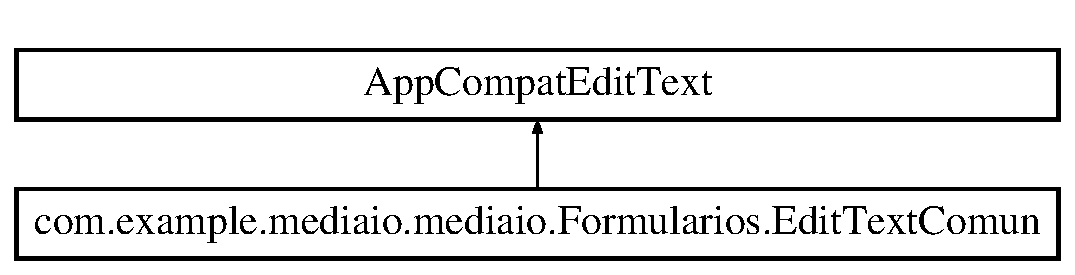
\includegraphics[height=2.000000cm]{classcom_1_1example_1_1mediaio_1_1mediaio_1_1_formularios_1_1_edit_text_comun}
\end{center}
\end{figure}
\subsection*{Métodos públicos}
\begin{DoxyCompactItemize}
\item 
\mbox{\Hypertarget{classcom_1_1example_1_1mediaio_1_1mediaio_1_1_formularios_1_1_edit_text_comun_a6540ab7d52b91de4b10ba70797bd3620}\label{classcom_1_1example_1_1mediaio_1_1mediaio_1_1_formularios_1_1_edit_text_comun_a6540ab7d52b91de4b10ba70797bd3620}} 
{\bfseries Edit\+Text\+Comun} (Context context)
\item 
\mbox{\Hypertarget{classcom_1_1example_1_1mediaio_1_1mediaio_1_1_formularios_1_1_edit_text_comun_ab703d109f9aad8c2f986b82dce737781}\label{classcom_1_1example_1_1mediaio_1_1mediaio_1_1_formularios_1_1_edit_text_comun_ab703d109f9aad8c2f986b82dce737781}} 
{\bfseries Edit\+Text\+Comun} (Context context, Attribute\+Set attrs)
\item 
\mbox{\Hypertarget{classcom_1_1example_1_1mediaio_1_1mediaio_1_1_formularios_1_1_edit_text_comun_a41ec48b6e34c5d643d585fe1fd510584}\label{classcom_1_1example_1_1mediaio_1_1mediaio_1_1_formularios_1_1_edit_text_comun_a41ec48b6e34c5d643d585fe1fd510584}} 
{\bfseries Edit\+Text\+Comun} (Context context, Attribute\+Set attrs, int def\+Style)
\item 
\mbox{\Hypertarget{classcom_1_1example_1_1mediaio_1_1mediaio_1_1_formularios_1_1_edit_text_comun_ab18dd4b107978146c636eb586f0710d7}\label{classcom_1_1example_1_1mediaio_1_1mediaio_1_1_formularios_1_1_edit_text_comun_ab18dd4b107978146c636eb586f0710d7}} 
String {\bfseries obtener\+Texto} ()  throws Input\+Erronea     
\end{DoxyCompactItemize}


\subsection{Descripción detallada}
Created by Marcos on 05/04/2017. 

La documentación para esta clase fue generada a partir del siguiente fichero\+:\begin{DoxyCompactItemize}
\item 
E\+:/\+Users/\+Marcos/\+Android\+Studio\+Projects/\+Media.\+io/app/src/main/java/com/example/mediaio/mediaio/\+Formularios/Edit\+Text\+Comun.\+java\end{DoxyCompactItemize}

\hypertarget{classcom_1_1example_1_1mediaio_1_1mediaio_1_1_formularios_1_1_edit_text_email}{}\section{Referencia de la Clase com.\+example.\+mediaio.\+mediaio.\+Formularios.\+Edit\+Text\+Email}
\label{classcom_1_1example_1_1mediaio_1_1mediaio_1_1_formularios_1_1_edit_text_email}\index{com.\+example.\+mediaio.\+mediaio.\+Formularios.\+Edit\+Text\+Email@{com.\+example.\+mediaio.\+mediaio.\+Formularios.\+Edit\+Text\+Email}}
Diagrama de herencias de com.\+example.\+mediaio.\+mediaio.\+Formularios.\+Edit\+Text\+Email\begin{figure}[H]
\begin{center}
\leavevmode
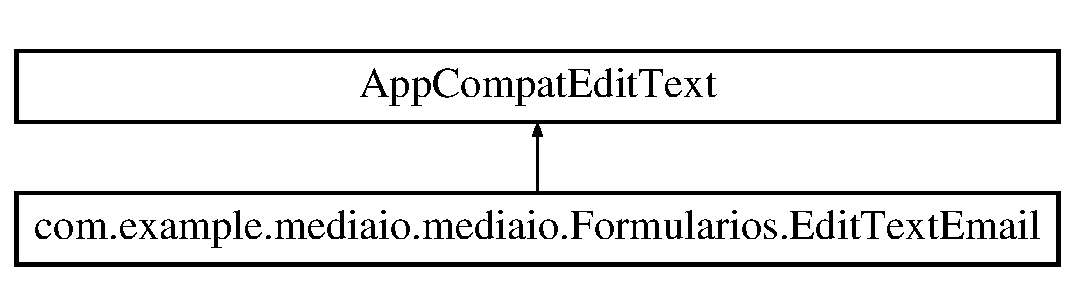
\includegraphics[height=2.000000cm]{classcom_1_1example_1_1mediaio_1_1mediaio_1_1_formularios_1_1_edit_text_email}
\end{center}
\end{figure}
\subsection*{Métodos públicos}
\begin{DoxyCompactItemize}
\item 
\mbox{\Hypertarget{classcom_1_1example_1_1mediaio_1_1mediaio_1_1_formularios_1_1_edit_text_email_a7d956f6545237fbc236d9f30d363e05d}\label{classcom_1_1example_1_1mediaio_1_1mediaio_1_1_formularios_1_1_edit_text_email_a7d956f6545237fbc236d9f30d363e05d}} 
{\bfseries Edit\+Text\+Email} (Context context)
\item 
\mbox{\Hypertarget{classcom_1_1example_1_1mediaio_1_1mediaio_1_1_formularios_1_1_edit_text_email_a9fd943561e03d4c67fffa9a460f113e1}\label{classcom_1_1example_1_1mediaio_1_1mediaio_1_1_formularios_1_1_edit_text_email_a9fd943561e03d4c67fffa9a460f113e1}} 
{\bfseries Edit\+Text\+Email} (Context context, Attribute\+Set attrs)
\item 
\mbox{\Hypertarget{classcom_1_1example_1_1mediaio_1_1mediaio_1_1_formularios_1_1_edit_text_email_aaee93af968f79ddb5a1db8e6440f9f03}\label{classcom_1_1example_1_1mediaio_1_1mediaio_1_1_formularios_1_1_edit_text_email_aaee93af968f79ddb5a1db8e6440f9f03}} 
{\bfseries Edit\+Text\+Email} (Context context, Attribute\+Set attrs, int def\+Style)
\item 
\mbox{\Hypertarget{classcom_1_1example_1_1mediaio_1_1mediaio_1_1_formularios_1_1_edit_text_email_adbe98bce2439899d972af33a7ee786ad}\label{classcom_1_1example_1_1mediaio_1_1mediaio_1_1_formularios_1_1_edit_text_email_adbe98bce2439899d972af33a7ee786ad}} 
boolean {\bfseries verificar} ()
\item 
\mbox{\Hypertarget{classcom_1_1example_1_1mediaio_1_1mediaio_1_1_formularios_1_1_edit_text_email_a2eaf2fdcb95e45a68e9fc9df91ecb717}\label{classcom_1_1example_1_1mediaio_1_1mediaio_1_1_formularios_1_1_edit_text_email_a2eaf2fdcb95e45a68e9fc9df91ecb717}} 
String {\bfseries obtener\+Texto} ()  throws Input\+Erronea     
\end{DoxyCompactItemize}


\subsection{Descripción detallada}
Created by Marcos on 05/04/2017. 

La documentación para esta clase fue generada a partir del siguiente fichero\+:\begin{DoxyCompactItemize}
\item 
E\+:/\+Users/\+Marcos/\+Android\+Studio\+Projects/\+Media.\+io/app/src/main/java/com/example/mediaio/mediaio/\+Formularios/Edit\+Text\+Email.\+java\end{DoxyCompactItemize}

\hypertarget{classcom_1_1example_1_1mediaio_1_1mediaio_1_1_formularios_1_1_edit_text_fecha}{}\section{Referencia de la Clase com.\+example.\+mediaio.\+mediaio.\+Formularios.\+Edit\+Text\+Fecha}
\label{classcom_1_1example_1_1mediaio_1_1mediaio_1_1_formularios_1_1_edit_text_fecha}\index{com.\+example.\+mediaio.\+mediaio.\+Formularios.\+Edit\+Text\+Fecha@{com.\+example.\+mediaio.\+mediaio.\+Formularios.\+Edit\+Text\+Fecha}}
Diagrama de herencias de com.\+example.\+mediaio.\+mediaio.\+Formularios.\+Edit\+Text\+Fecha\begin{figure}[H]
\begin{center}
\leavevmode
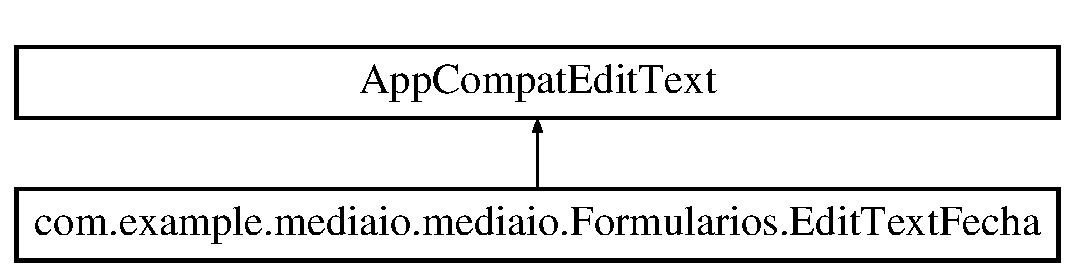
\includegraphics[height=2.000000cm]{classcom_1_1example_1_1mediaio_1_1mediaio_1_1_formularios_1_1_edit_text_fecha}
\end{center}
\end{figure}
\subsection*{Métodos públicos}
\begin{DoxyCompactItemize}
\item 
\mbox{\Hypertarget{classcom_1_1example_1_1mediaio_1_1mediaio_1_1_formularios_1_1_edit_text_fecha_a3429ce06c4e3926fd7784ba221cc8f40}\label{classcom_1_1example_1_1mediaio_1_1mediaio_1_1_formularios_1_1_edit_text_fecha_a3429ce06c4e3926fd7784ba221cc8f40}} 
{\bfseries Edit\+Text\+Fecha} (Context context)
\item 
\mbox{\Hypertarget{classcom_1_1example_1_1mediaio_1_1mediaio_1_1_formularios_1_1_edit_text_fecha_a1c8eab5de33c465974eac7f5b627898a}\label{classcom_1_1example_1_1mediaio_1_1mediaio_1_1_formularios_1_1_edit_text_fecha_a1c8eab5de33c465974eac7f5b627898a}} 
{\bfseries Edit\+Text\+Fecha} (Context context, Attribute\+Set attrs)
\item 
\mbox{\Hypertarget{classcom_1_1example_1_1mediaio_1_1mediaio_1_1_formularios_1_1_edit_text_fecha_ad0833582518d89718bd43dd1ce13edb5}\label{classcom_1_1example_1_1mediaio_1_1mediaio_1_1_formularios_1_1_edit_text_fecha_ad0833582518d89718bd43dd1ce13edb5}} 
{\bfseries Edit\+Text\+Fecha} (Context context, Attribute\+Set attrs, int def\+Style)
\item 
\mbox{\Hypertarget{classcom_1_1example_1_1mediaio_1_1mediaio_1_1_formularios_1_1_edit_text_fecha_a0942a50af68eda2f0b2ced126a3a937b}\label{classcom_1_1example_1_1mediaio_1_1mediaio_1_1_formularios_1_1_edit_text_fecha_a0942a50af68eda2f0b2ced126a3a937b}} 
boolean {\bfseries verificar} ()
\item 
\mbox{\Hypertarget{classcom_1_1example_1_1mediaio_1_1mediaio_1_1_formularios_1_1_edit_text_fecha_a7cedad62657a08663dd46f45107cf2a5}\label{classcom_1_1example_1_1mediaio_1_1mediaio_1_1_formularios_1_1_edit_text_fecha_a7cedad62657a08663dd46f45107cf2a5}} 
String {\bfseries obtener\+Texto} ()  throws Input\+Erronea     
\end{DoxyCompactItemize}


\subsection{Descripción detallada}
Created by Marcos on 05/04/2017. 

La documentación para esta clase fue generada a partir del siguiente fichero\+:\begin{DoxyCompactItemize}
\item 
E\+:/\+Users/\+Marcos/\+Android\+Studio\+Projects/\+Media.\+io/app/src/main/java/com/example/mediaio/mediaio/\+Formularios/Edit\+Text\+Fecha.\+java\end{DoxyCompactItemize}

\hypertarget{classcom_1_1example_1_1mediaio_1_1mediaio_1_1_formularios_1_1_edit_text_password}{}\section{Referencia de la Clase com.\+example.\+mediaio.\+mediaio.\+Formularios.\+Edit\+Text\+Password}
\label{classcom_1_1example_1_1mediaio_1_1mediaio_1_1_formularios_1_1_edit_text_password}\index{com.\+example.\+mediaio.\+mediaio.\+Formularios.\+Edit\+Text\+Password@{com.\+example.\+mediaio.\+mediaio.\+Formularios.\+Edit\+Text\+Password}}
Diagrama de herencias de com.\+example.\+mediaio.\+mediaio.\+Formularios.\+Edit\+Text\+Password\begin{figure}[H]
\begin{center}
\leavevmode
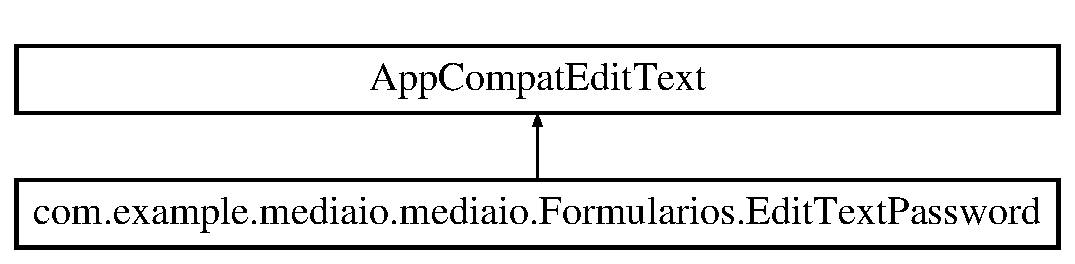
\includegraphics[height=2.000000cm]{classcom_1_1example_1_1mediaio_1_1mediaio_1_1_formularios_1_1_edit_text_password}
\end{center}
\end{figure}
\subsection*{Métodos públicos}
\begin{DoxyCompactItemize}
\item 
\mbox{\Hypertarget{classcom_1_1example_1_1mediaio_1_1mediaio_1_1_formularios_1_1_edit_text_password_a96dba8342aa6e151d35646019243f469}\label{classcom_1_1example_1_1mediaio_1_1mediaio_1_1_formularios_1_1_edit_text_password_a96dba8342aa6e151d35646019243f469}} 
{\bfseries Edit\+Text\+Password} (Context context)
\item 
\mbox{\Hypertarget{classcom_1_1example_1_1mediaio_1_1mediaio_1_1_formularios_1_1_edit_text_password_af9ffd043b33e50ac3d93371581ed385d}\label{classcom_1_1example_1_1mediaio_1_1mediaio_1_1_formularios_1_1_edit_text_password_af9ffd043b33e50ac3d93371581ed385d}} 
{\bfseries Edit\+Text\+Password} (Context context, Attribute\+Set attrs)
\item 
\mbox{\Hypertarget{classcom_1_1example_1_1mediaio_1_1mediaio_1_1_formularios_1_1_edit_text_password_ae43d621ba5454194869855f5fa6e4c6b}\label{classcom_1_1example_1_1mediaio_1_1mediaio_1_1_formularios_1_1_edit_text_password_ae43d621ba5454194869855f5fa6e4c6b}} 
{\bfseries Edit\+Text\+Password} (Context context, Attribute\+Set attrs, int def\+Style)
\item 
\mbox{\Hypertarget{classcom_1_1example_1_1mediaio_1_1mediaio_1_1_formularios_1_1_edit_text_password_a4b2eab7bdbef01a1da4a79a4a68a34bf}\label{classcom_1_1example_1_1mediaio_1_1mediaio_1_1_formularios_1_1_edit_text_password_a4b2eab7bdbef01a1da4a79a4a68a34bf}} 
boolean {\bfseries verificar} ()
\item 
\mbox{\Hypertarget{classcom_1_1example_1_1mediaio_1_1mediaio_1_1_formularios_1_1_edit_text_password_a363944d321bd3af5077d7dfd60263078}\label{classcom_1_1example_1_1mediaio_1_1mediaio_1_1_formularios_1_1_edit_text_password_a363944d321bd3af5077d7dfd60263078}} 
String {\bfseries obtener\+Texto} ()  throws Input\+Erronea     
\end{DoxyCompactItemize}


\subsection{Descripción detallada}
Created by Marcos on 05/04/2017. 

La documentación para esta clase fue generada a partir del siguiente fichero\+:\begin{DoxyCompactItemize}
\item 
E\+:/\+Users/\+Marcos/\+Android\+Studio\+Projects/\+Media.\+io/app/src/main/java/com/example/mediaio/mediaio/\+Formularios/Edit\+Text\+Password.\+java\end{DoxyCompactItemize}

\hypertarget{classcom_1_1example_1_1mediaio_1_1mediaio_1_1_excepciones_1_1_input_erronea}{}\section{Referencia de la Clase com.\+example.\+mediaio.\+mediaio.\+Excepciones.\+Input\+Erronea}
\label{classcom_1_1example_1_1mediaio_1_1mediaio_1_1_excepciones_1_1_input_erronea}\index{com.\+example.\+mediaio.\+mediaio.\+Excepciones.\+Input\+Erronea@{com.\+example.\+mediaio.\+mediaio.\+Excepciones.\+Input\+Erronea}}
Diagrama de herencias de com.\+example.\+mediaio.\+mediaio.\+Excepciones.\+Input\+Erronea\begin{figure}[H]
\begin{center}
\leavevmode
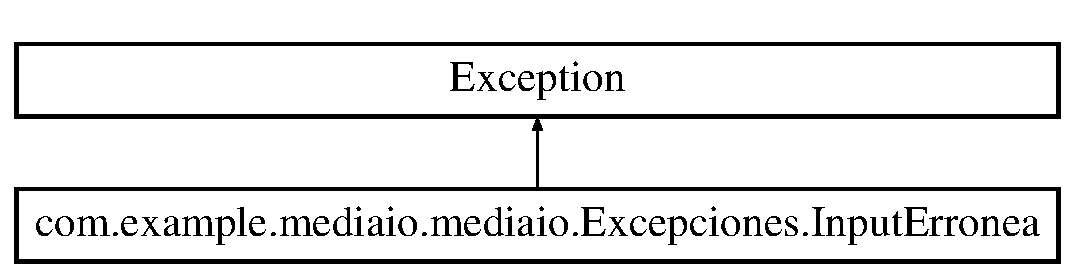
\includegraphics[height=2.000000cm]{classcom_1_1example_1_1mediaio_1_1mediaio_1_1_excepciones_1_1_input_erronea}
\end{center}
\end{figure}


\subsection{Descripción detallada}
Created by Marcos on 05/04/2017. 

La documentación para esta clase fue generada a partir del siguiente fichero\+:\begin{DoxyCompactItemize}
\item 
E\+:/\+Users/\+Marcos/\+Android\+Studio\+Projects/\+Media.\+io/app/src/main/java/com/example/mediaio/mediaio/\+Excepciones/Input\+Erronea.\+java\end{DoxyCompactItemize}

\hypertarget{classcom_1_1example_1_1mediaio_1_1mediaio_1_1modelo_1_1_interfaz_rest}{}\section{Referencia de la Clase com.\+example.\+mediaio.\+mediaio.\+modelo.\+Interfaz\+Rest}
\label{classcom_1_1example_1_1mediaio_1_1mediaio_1_1modelo_1_1_interfaz_rest}\index{com.\+example.\+mediaio.\+mediaio.\+modelo.\+Interfaz\+Rest@{com.\+example.\+mediaio.\+mediaio.\+modelo.\+Interfaz\+Rest}}
Diagrama de herencias de com.\+example.\+mediaio.\+mediaio.\+modelo.\+Interfaz\+Rest\begin{figure}[H]
\begin{center}
\leavevmode
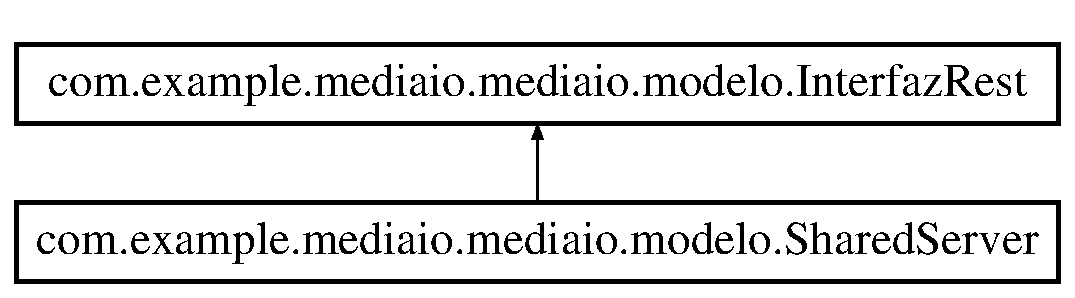
\includegraphics[height=2.000000cm]{classcom_1_1example_1_1mediaio_1_1mediaio_1_1modelo_1_1_interfaz_rest}
\end{center}
\end{figure}
\subsection*{Métodos protegidos}
\begin{DoxyCompactItemize}
\item 
\mbox{\Hypertarget{classcom_1_1example_1_1mediaio_1_1mediaio_1_1modelo_1_1_interfaz_rest_aa8a213a667ad5f0cc7ef8af1aedebb6c}\label{classcom_1_1example_1_1mediaio_1_1mediaio_1_1modelo_1_1_interfaz_rest_aa8a213a667ad5f0cc7ef8af1aedebb6c}} 
void {\bfseries enviar\+P\+O\+ST} (final String U\+RL, final J\+S\+O\+N\+Object json, final \hyperlink{classcom_1_1example_1_1mediaio_1_1mediaio_1_1modelo_1_1_j_s_o_n_callback}{J\+S\+O\+N\+Callback} callback)
\item 
\mbox{\Hypertarget{classcom_1_1example_1_1mediaio_1_1mediaio_1_1modelo_1_1_interfaz_rest_afd3b5f37bb77a9d6921038e7675869fe}\label{classcom_1_1example_1_1mediaio_1_1mediaio_1_1modelo_1_1_interfaz_rest_afd3b5f37bb77a9d6921038e7675869fe}} 
void {\bfseries enviar\+G\+ET} (final String U\+RL, final \hyperlink{classcom_1_1example_1_1mediaio_1_1mediaio_1_1modelo_1_1_j_s_o_n_callback}{J\+S\+O\+N\+Callback} callback)
\end{DoxyCompactItemize}


\subsection{Descripción detallada}
Created by Marcos on 01/04/2017. 

La documentación para esta clase fue generada a partir del siguiente fichero\+:\begin{DoxyCompactItemize}
\item 
E\+:/\+Users/\+Marcos/\+Android\+Studio\+Projects/\+Media.\+io/app/src/main/java/com/example/mediaio/mediaio/modelo/Interfaz\+Rest.\+java\end{DoxyCompactItemize}

\hypertarget{classcom_1_1example_1_1mediaio_1_1mediaio_1_1modelo_1_1_j_s_o_n_callback}{}\section{Referencia de la Clase com.\+example.\+mediaio.\+mediaio.\+modelo.\+J\+S\+O\+N\+Callback}
\label{classcom_1_1example_1_1mediaio_1_1mediaio_1_1modelo_1_1_j_s_o_n_callback}\index{com.\+example.\+mediaio.\+mediaio.\+modelo.\+J\+S\+O\+N\+Callback@{com.\+example.\+mediaio.\+mediaio.\+modelo.\+J\+S\+O\+N\+Callback}}
Diagrama de herencias de com.\+example.\+mediaio.\+mediaio.\+modelo.\+J\+S\+O\+N\+Callback\begin{figure}[H]
\begin{center}
\leavevmode
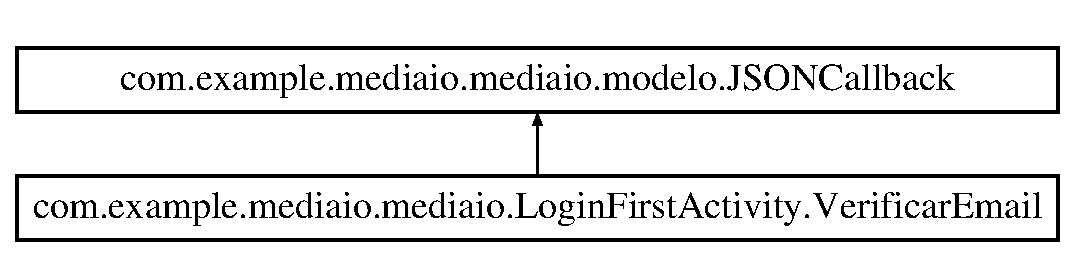
\includegraphics[height=2.000000cm]{classcom_1_1example_1_1mediaio_1_1mediaio_1_1modelo_1_1_j_s_o_n_callback}
\end{center}
\end{figure}
\subsection*{Métodos públicos}
\begin{DoxyCompactItemize}
\item 
\mbox{\Hypertarget{classcom_1_1example_1_1mediaio_1_1mediaio_1_1modelo_1_1_j_s_o_n_callback_a3058429efea086b6579aaec145619ed4}\label{classcom_1_1example_1_1mediaio_1_1mediaio_1_1modelo_1_1_j_s_o_n_callback_a3058429efea086b6579aaec145619ed4}} 
abstract void {\bfseries ejecutar} (J\+S\+O\+N\+Object respuesta, long codigo\+Servidor)
\end{DoxyCompactItemize}


\subsection{Descripción detallada}
Created by Marcos on 01/04/2017. 

La documentación para esta clase fue generada a partir del siguiente fichero\+:\begin{DoxyCompactItemize}
\item 
E\+:/\+Users/\+Marcos/\+Android\+Studio\+Projects/\+Media.\+io/app/src/main/java/com/example/mediaio/mediaio/modelo/J\+S\+O\+N\+Callback.\+java\end{DoxyCompactItemize}

\hypertarget{classcom_1_1example_1_1mediaio_1_1mediaio_1_1_login_first_activity}{}\section{Referencia de la Clase com.\+example.\+mediaio.\+mediaio.\+Login\+First\+Activity}
\label{classcom_1_1example_1_1mediaio_1_1mediaio_1_1_login_first_activity}\index{com.\+example.\+mediaio.\+mediaio.\+Login\+First\+Activity@{com.\+example.\+mediaio.\+mediaio.\+Login\+First\+Activity}}
Diagrama de herencias de com.\+example.\+mediaio.\+mediaio.\+Login\+First\+Activity\begin{figure}[H]
\begin{center}
\leavevmode
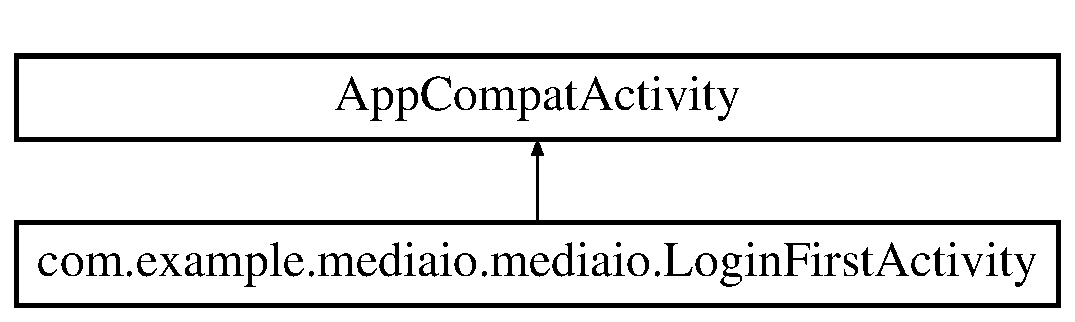
\includegraphics[height=2.000000cm]{classcom_1_1example_1_1mediaio_1_1mediaio_1_1_login_first_activity}
\end{center}
\end{figure}
\subsection*{Clases}
\begin{DoxyCompactItemize}
\item 
class \hyperlink{classcom_1_1example_1_1mediaio_1_1mediaio_1_1_login_first_activity_1_1_verificar_email}{Verificar\+Email}
\end{DoxyCompactItemize}
\subsection*{Métodos protegidos}
\begin{DoxyCompactItemize}
\item 
\mbox{\Hypertarget{classcom_1_1example_1_1mediaio_1_1mediaio_1_1_login_first_activity_a460f89d7dacaeb22ff9487c29d6362d7}\label{classcom_1_1example_1_1mediaio_1_1mediaio_1_1_login_first_activity_a460f89d7dacaeb22ff9487c29d6362d7}} 
void {\bfseries on\+Create} (Bundle saved\+Instance\+State)
\item 
\mbox{\Hypertarget{classcom_1_1example_1_1mediaio_1_1mediaio_1_1_login_first_activity_a9c3759d6bc6d41c5dfaba30eb2b89df0}\label{classcom_1_1example_1_1mediaio_1_1mediaio_1_1_login_first_activity_a9c3759d6bc6d41c5dfaba30eb2b89df0}} 
void {\bfseries on\+Activity\+Result} (int request\+Code, int result\+Code, Intent data)
\end{DoxyCompactItemize}


La documentación para esta clase fue generada a partir del siguiente fichero\+:\begin{DoxyCompactItemize}
\item 
E\+:/\+Users/\+Marcos/\+Android\+Studio\+Projects/\+Media.\+io/app/src/main/java/com/example/mediaio/mediaio/Login\+First\+Activity.\+java\end{DoxyCompactItemize}

\hypertarget{classcom_1_1example_1_1mediaio_1_1mediaio_1_1_login_second_activity}{}\section{Referencia de la Clase com.\+example.\+mediaio.\+mediaio.\+Login\+Second\+Activity}
\label{classcom_1_1example_1_1mediaio_1_1mediaio_1_1_login_second_activity}\index{com.\+example.\+mediaio.\+mediaio.\+Login\+Second\+Activity@{com.\+example.\+mediaio.\+mediaio.\+Login\+Second\+Activity}}
Diagrama de herencias de com.\+example.\+mediaio.\+mediaio.\+Login\+Second\+Activity\begin{figure}[H]
\begin{center}
\leavevmode
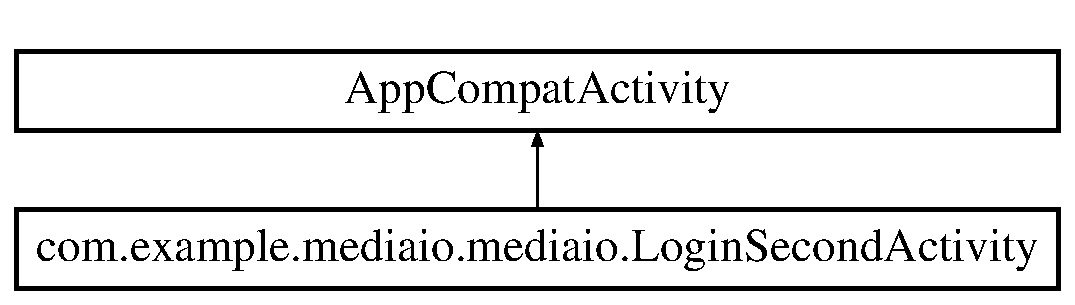
\includegraphics[height=2.000000cm]{classcom_1_1example_1_1mediaio_1_1mediaio_1_1_login_second_activity}
\end{center}
\end{figure}
\subsection*{Métodos protegidos}
\begin{DoxyCompactItemize}
\item 
\mbox{\Hypertarget{classcom_1_1example_1_1mediaio_1_1mediaio_1_1_login_second_activity_a3952a1aae2c3366a8318c075a3365494}\label{classcom_1_1example_1_1mediaio_1_1mediaio_1_1_login_second_activity_a3952a1aae2c3366a8318c075a3365494}} 
void {\bfseries on\+Create} (Bundle saved\+Instance\+State)
\end{DoxyCompactItemize}


La documentación para esta clase fue generada a partir del siguiente fichero\+:\begin{DoxyCompactItemize}
\item 
E\+:/\+Users/\+Marcos/\+Android\+Studio\+Projects/\+Media.\+io/app/src/main/java/com/example/mediaio/mediaio/Login\+Second\+Activity.\+java\end{DoxyCompactItemize}

\hypertarget{classcom_1_1example_1_1mediaio_1_1mediaio_1_1_main_activity}{}\section{Referencia de la Clase com.\+example.\+mediaio.\+mediaio.\+Main\+Activity}
\label{classcom_1_1example_1_1mediaio_1_1mediaio_1_1_main_activity}\index{com.\+example.\+mediaio.\+mediaio.\+Main\+Activity@{com.\+example.\+mediaio.\+mediaio.\+Main\+Activity}}
Diagrama de herencias de com.\+example.\+mediaio.\+mediaio.\+Main\+Activity\begin{figure}[H]
\begin{center}
\leavevmode
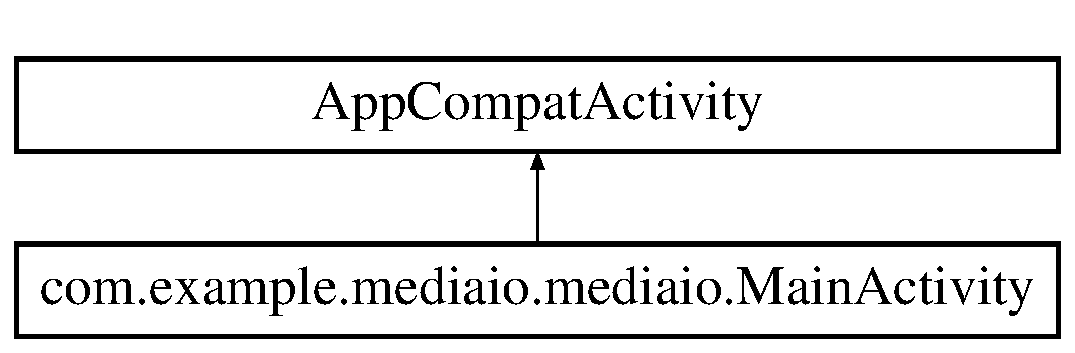
\includegraphics[height=2.000000cm]{classcom_1_1example_1_1mediaio_1_1mediaio_1_1_main_activity}
\end{center}
\end{figure}
\subsection*{Métodos protegidos}
\begin{DoxyCompactItemize}
\item 
\mbox{\Hypertarget{classcom_1_1example_1_1mediaio_1_1mediaio_1_1_main_activity_ac954ad02ab69c9eb698aa7b2c9de2488}\label{classcom_1_1example_1_1mediaio_1_1mediaio_1_1_main_activity_ac954ad02ab69c9eb698aa7b2c9de2488}} 
void {\bfseries on\+Create} (Bundle saved\+Instance\+State)
\end{DoxyCompactItemize}


La documentación para esta clase fue generada a partir del siguiente fichero\+:\begin{DoxyCompactItemize}
\item 
E\+:/\+Users/\+Marcos/\+Android\+Studio\+Projects/\+Media.\+io/app/src/main/java/com/example/mediaio/mediaio/Main\+Activity.\+java\end{DoxyCompactItemize}

\hypertarget{classcom_1_1example_1_1mediaio_1_1mediaio_1_1_media_i_o_chat}{}\section{Referencia de la Clase com.\+example.\+mediaio.\+mediaio.\+Media\+I\+O\+Chat}
\label{classcom_1_1example_1_1mediaio_1_1mediaio_1_1_media_i_o_chat}\index{com.\+example.\+mediaio.\+mediaio.\+Media\+I\+O\+Chat@{com.\+example.\+mediaio.\+mediaio.\+Media\+I\+O\+Chat}}
Diagrama de herencias de com.\+example.\+mediaio.\+mediaio.\+Media\+I\+O\+Chat\begin{figure}[H]
\begin{center}
\leavevmode
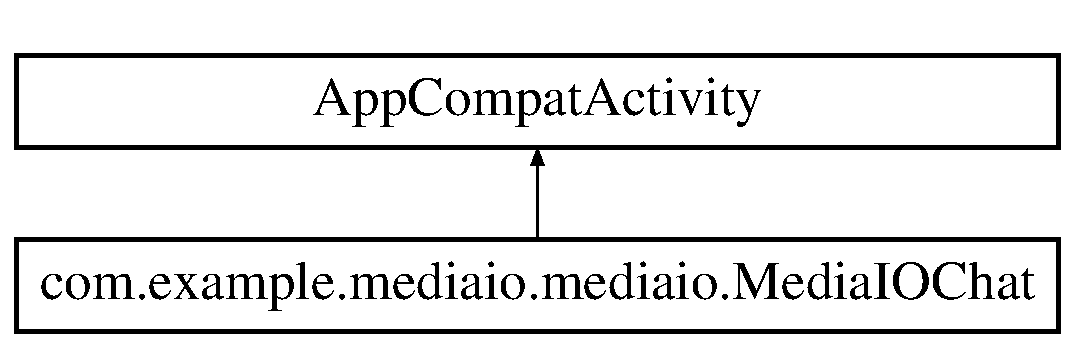
\includegraphics[height=2.000000cm]{classcom_1_1example_1_1mediaio_1_1mediaio_1_1_media_i_o_chat}
\end{center}
\end{figure}
\subsection*{Métodos protegidos}
\begin{DoxyCompactItemize}
\item 
\mbox{\Hypertarget{classcom_1_1example_1_1mediaio_1_1mediaio_1_1_media_i_o_chat_a6358cfbf22c5dc7531ed4836a647c879}\label{classcom_1_1example_1_1mediaio_1_1mediaio_1_1_media_i_o_chat_a6358cfbf22c5dc7531ed4836a647c879}} 
void {\bfseries on\+Create} (Bundle saved\+Instance\+State)
\end{DoxyCompactItemize}


La documentación para esta clase fue generada a partir del siguiente fichero\+:\begin{DoxyCompactItemize}
\item 
E\+:/\+Users/\+Marcos/\+Android\+Studio\+Projects/\+Media.\+io/app/src/main/java/com/example/mediaio/mediaio/Media\+I\+O\+Chat.\+java\end{DoxyCompactItemize}

\hypertarget{classcom_1_1example_1_1mediaio_1_1mediaio_1_1_media_i_o_main}{}\section{Referencia de la Clase com.\+example.\+mediaio.\+mediaio.\+Media\+I\+O\+Main}
\label{classcom_1_1example_1_1mediaio_1_1mediaio_1_1_media_i_o_main}\index{com.\+example.\+mediaio.\+mediaio.\+Media\+I\+O\+Main@{com.\+example.\+mediaio.\+mediaio.\+Media\+I\+O\+Main}}
Diagrama de herencias de com.\+example.\+mediaio.\+mediaio.\+Media\+I\+O\+Main\begin{figure}[H]
\begin{center}
\leavevmode
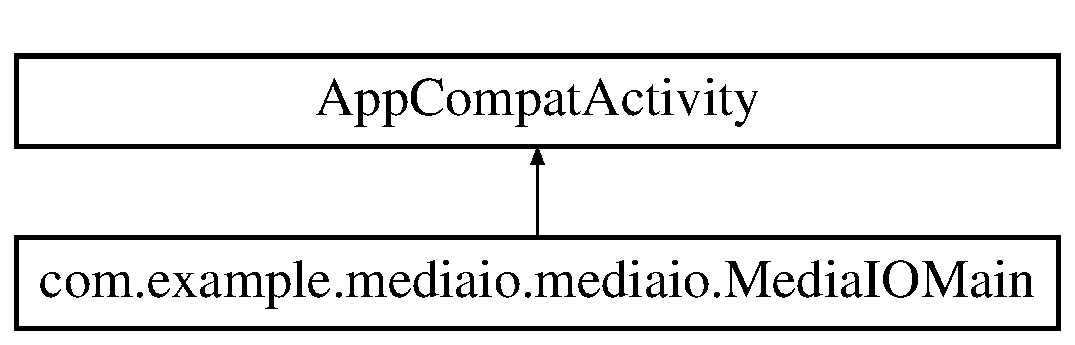
\includegraphics[height=2.000000cm]{classcom_1_1example_1_1mediaio_1_1mediaio_1_1_media_i_o_main}
\end{center}
\end{figure}
\subsection*{Métodos protegidos}
\begin{DoxyCompactItemize}
\item 
\mbox{\Hypertarget{classcom_1_1example_1_1mediaio_1_1mediaio_1_1_media_i_o_main_acb26bcbdec3a3c537c4d95a4f4caf07d}\label{classcom_1_1example_1_1mediaio_1_1mediaio_1_1_media_i_o_main_acb26bcbdec3a3c537c4d95a4f4caf07d}} 
void {\bfseries on\+Create} (Bundle saved\+Instance\+State)
\end{DoxyCompactItemize}


La documentación para esta clase fue generada a partir del siguiente fichero\+:\begin{DoxyCompactItemize}
\item 
E\+:/\+Users/\+Marcos/\+Android\+Studio\+Projects/\+Media.\+io/app/src/main/java/com/example/mediaio/mediaio/Media\+I\+O\+Main.\+java\end{DoxyCompactItemize}

\hypertarget{classcom_1_1example_1_1mediaio_1_1mediaio_1_1_media_i_o_perfil}{}\section{Referencia de la Clase com.\+example.\+mediaio.\+mediaio.\+Media\+I\+O\+Perfil}
\label{classcom_1_1example_1_1mediaio_1_1mediaio_1_1_media_i_o_perfil}\index{com.\+example.\+mediaio.\+mediaio.\+Media\+I\+O\+Perfil@{com.\+example.\+mediaio.\+mediaio.\+Media\+I\+O\+Perfil}}
Diagrama de herencias de com.\+example.\+mediaio.\+mediaio.\+Media\+I\+O\+Perfil\begin{figure}[H]
\begin{center}
\leavevmode
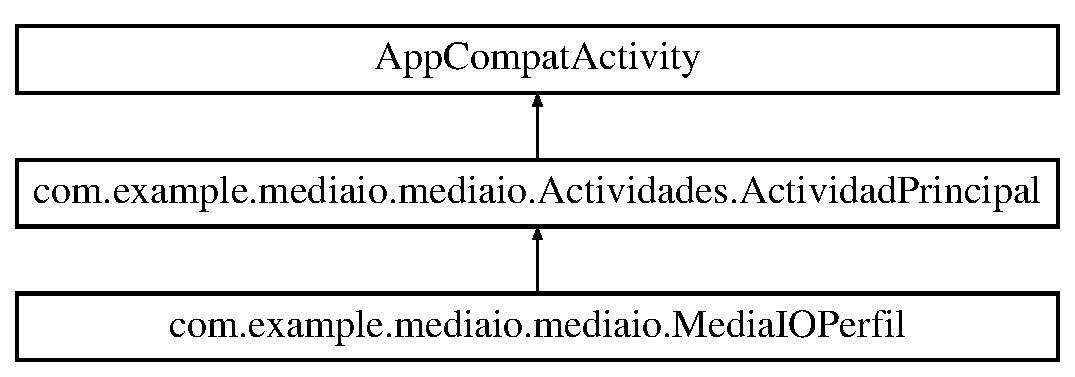
\includegraphics[height=3.000000cm]{classcom_1_1example_1_1mediaio_1_1mediaio_1_1_media_i_o_perfil}
\end{center}
\end{figure}
\subsection*{Métodos protegidos}
\begin{DoxyCompactItemize}
\item 
\mbox{\Hypertarget{classcom_1_1example_1_1mediaio_1_1mediaio_1_1_media_i_o_perfil_a800db037e22311f3490a9ff9d8f36e50}\label{classcom_1_1example_1_1mediaio_1_1mediaio_1_1_media_i_o_perfil_a800db037e22311f3490a9ff9d8f36e50}} 
void {\bfseries on\+Create} (Bundle saved\+Instance\+State)
\item 
\mbox{\Hypertarget{classcom_1_1example_1_1mediaio_1_1mediaio_1_1_media_i_o_perfil_ade7cb61e291925f56204763b8d7d4409}\label{classcom_1_1example_1_1mediaio_1_1mediaio_1_1_media_i_o_perfil_ade7cb61e291925f56204763b8d7d4409}} 
void {\bfseries on\+Activity\+Result} (int request\+Code, int result\+Code, Intent data)
\end{DoxyCompactItemize}
\subsection*{Otros miembros heredados}


La documentación para esta clase fue generada a partir del siguiente fichero\+:\begin{DoxyCompactItemize}
\item 
E\+:/\+Users/\+Marcos/\+Android\+Studio\+Projects/\+Media.\+io/app/src/main/java/com/example/mediaio/mediaio/Media\+I\+O\+Perfil.\+java\end{DoxyCompactItemize}

\hypertarget{classcom_1_1example_1_1mediaio_1_1mediaio_1_1_media_i_o_play}{}\section{Referencia de la Clase com.\+example.\+mediaio.\+mediaio.\+Media\+I\+O\+Play}
\label{classcom_1_1example_1_1mediaio_1_1mediaio_1_1_media_i_o_play}\index{com.\+example.\+mediaio.\+mediaio.\+Media\+I\+O\+Play@{com.\+example.\+mediaio.\+mediaio.\+Media\+I\+O\+Play}}
Diagrama de herencias de com.\+example.\+mediaio.\+mediaio.\+Media\+I\+O\+Play\begin{figure}[H]
\begin{center}
\leavevmode
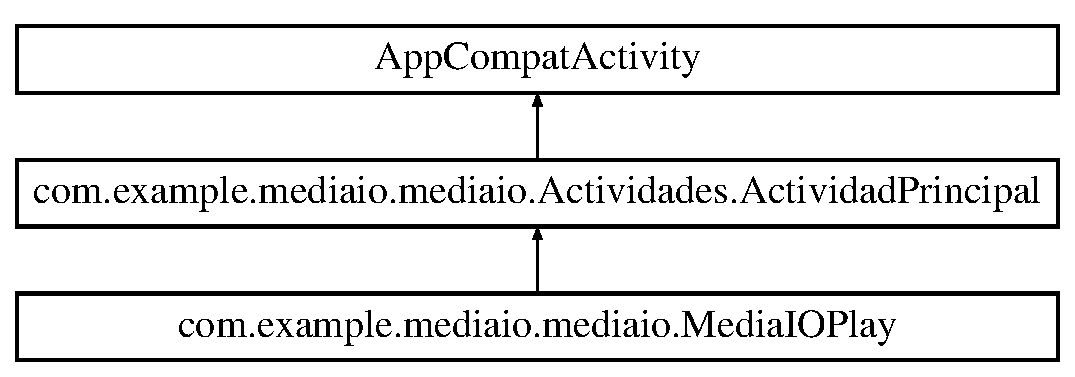
\includegraphics[height=3.000000cm]{classcom_1_1example_1_1mediaio_1_1mediaio_1_1_media_i_o_play}
\end{center}
\end{figure}
\subsection*{Métodos protegidos}
\begin{DoxyCompactItemize}
\item 
\mbox{\Hypertarget{classcom_1_1example_1_1mediaio_1_1mediaio_1_1_media_i_o_play_a8d734a36933c7f26b4b2d77453f74d94}\label{classcom_1_1example_1_1mediaio_1_1mediaio_1_1_media_i_o_play_a8d734a36933c7f26b4b2d77453f74d94}} 
void {\bfseries on\+Create} (Bundle saved\+Instance\+State)
\end{DoxyCompactItemize}
\subsection*{Otros miembros heredados}


La documentación para esta clase fue generada a partir del siguiente fichero\+:\begin{DoxyCompactItemize}
\item 
E\+:/\+Users/\+Marcos/\+Android\+Studio\+Projects/\+Media.\+io/app/src/main/java/com/example/mediaio/mediaio/Media\+I\+O\+Play.\+java\end{DoxyCompactItemize}

\hypertarget{classcom_1_1example_1_1mediaio_1_1mediaio_1_1_media_i_o_registrar}{}\section{Referencia de la Clase com.\+example.\+mediaio.\+mediaio.\+Media\+I\+O\+Registrar}
\label{classcom_1_1example_1_1mediaio_1_1mediaio_1_1_media_i_o_registrar}\index{com.\+example.\+mediaio.\+mediaio.\+Media\+I\+O\+Registrar@{com.\+example.\+mediaio.\+mediaio.\+Media\+I\+O\+Registrar}}
Diagrama de herencias de com.\+example.\+mediaio.\+mediaio.\+Media\+I\+O\+Registrar\begin{figure}[H]
\begin{center}
\leavevmode
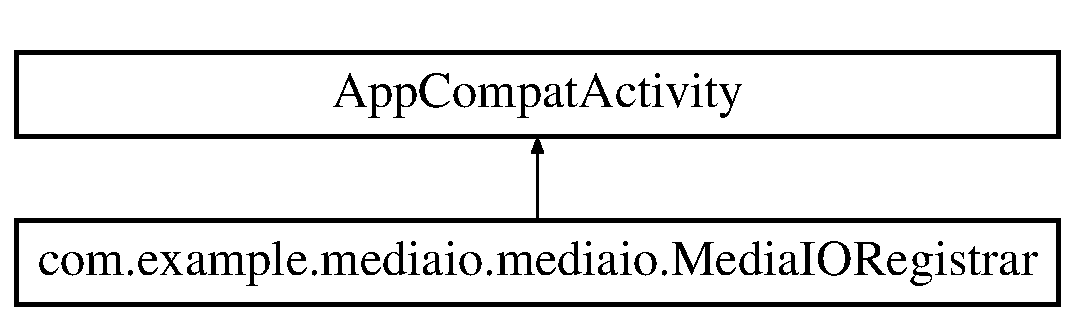
\includegraphics[height=2.000000cm]{classcom_1_1example_1_1mediaio_1_1mediaio_1_1_media_i_o_registrar}
\end{center}
\end{figure}
\subsection*{Métodos protegidos}
\begin{DoxyCompactItemize}
\item 
\mbox{\Hypertarget{classcom_1_1example_1_1mediaio_1_1mediaio_1_1_media_i_o_registrar_aeb92c6562f9938323bbafe38560fec8f}\label{classcom_1_1example_1_1mediaio_1_1mediaio_1_1_media_i_o_registrar_aeb92c6562f9938323bbafe38560fec8f}} 
void {\bfseries on\+Create} (Bundle saved\+Instance\+State)
\item 
\mbox{\Hypertarget{classcom_1_1example_1_1mediaio_1_1mediaio_1_1_media_i_o_registrar_a99606f48de21b8998c340cb2120359b0}\label{classcom_1_1example_1_1mediaio_1_1mediaio_1_1_media_i_o_registrar_a99606f48de21b8998c340cb2120359b0}} 
void {\bfseries on\+Activity\+Result} (int request\+Code, int result\+Code, Intent data)
\end{DoxyCompactItemize}


La documentación para esta clase fue generada a partir del siguiente fichero\+:\begin{DoxyCompactItemize}
\item 
E\+:/\+Users/\+Marcos/\+Android\+Studio\+Projects/\+Media.\+io/app/src/main/java/com/example/mediaio/mediaio/Media\+I\+O\+Registrar.\+java\end{DoxyCompactItemize}

\hypertarget{classcom_1_1example_1_1mediaio_1_1mediaio_1_1modelo_1_1_mensaje_firebase}{}\section{Referencia de la Clase com.\+example.\+mediaio.\+mediaio.\+modelo.\+Mensaje\+Firebase}
\label{classcom_1_1example_1_1mediaio_1_1mediaio_1_1modelo_1_1_mensaje_firebase}\index{com.\+example.\+mediaio.\+mediaio.\+modelo.\+Mensaje\+Firebase@{com.\+example.\+mediaio.\+mediaio.\+modelo.\+Mensaje\+Firebase}}
\subsection*{Métodos públicos}
\begin{DoxyCompactItemize}
\item 
\mbox{\Hypertarget{classcom_1_1example_1_1mediaio_1_1mediaio_1_1modelo_1_1_mensaje_firebase_a7f5074b5f9a9b3692bd90b2fd2f037b8}\label{classcom_1_1example_1_1mediaio_1_1mediaio_1_1modelo_1_1_mensaje_firebase_a7f5074b5f9a9b3692bd90b2fd2f037b8}} 
{\bfseries Mensaje\+Firebase} (String texto, String usuario)
\end{DoxyCompactItemize}
\subsection*{Atributos públicos}
\begin{DoxyCompactItemize}
\item 
\mbox{\Hypertarget{classcom_1_1example_1_1mediaio_1_1mediaio_1_1modelo_1_1_mensaje_firebase_ad0458999666994872769e63bb9401b03}\label{classcom_1_1example_1_1mediaio_1_1mediaio_1_1modelo_1_1_mensaje_firebase_ad0458999666994872769e63bb9401b03}} 
String {\bfseries texto}
\item 
\mbox{\Hypertarget{classcom_1_1example_1_1mediaio_1_1mediaio_1_1modelo_1_1_mensaje_firebase_aa3ff15def368052a2adc3a29b18f35b4}\label{classcom_1_1example_1_1mediaio_1_1mediaio_1_1modelo_1_1_mensaje_firebase_aa3ff15def368052a2adc3a29b18f35b4}} 
String {\bfseries usuario}
\item 
\mbox{\Hypertarget{classcom_1_1example_1_1mediaio_1_1mediaio_1_1modelo_1_1_mensaje_firebase_a5bf7de4bf4b3a8526f01c77d2435d6ac}\label{classcom_1_1example_1_1mediaio_1_1mediaio_1_1modelo_1_1_mensaje_firebase_a5bf7de4bf4b3a8526f01c77d2435d6ac}} 
long {\bfseries timestamp}
\end{DoxyCompactItemize}


\subsection{Descripción detallada}
Created by Marcos on 26/04/2017. 

La documentación para esta clase fue generada a partir del siguiente fichero\+:\begin{DoxyCompactItemize}
\item 
E\+:/\+Users/\+Marcos/\+Android\+Studio\+Projects/\+Media.\+io/app/src/main/java/com/example/mediaio/mediaio/modelo/Mensaje\+Firebase.\+java\end{DoxyCompactItemize}

\hypertarget{classcom_1_1example_1_1mediaio_1_1mediaio_1_1modelo_1_1_reproductor}{}\section{Referencia de la Clase com.\+example.\+mediaio.\+mediaio.\+modelo.\+Reproductor}
\label{classcom_1_1example_1_1mediaio_1_1mediaio_1_1modelo_1_1_reproductor}\index{com.\+example.\+mediaio.\+mediaio.\+modelo.\+Reproductor@{com.\+example.\+mediaio.\+mediaio.\+modelo.\+Reproductor}}
Diagrama de herencias de com.\+example.\+mediaio.\+mediaio.\+modelo.\+Reproductor\begin{figure}[H]
\begin{center}
\leavevmode
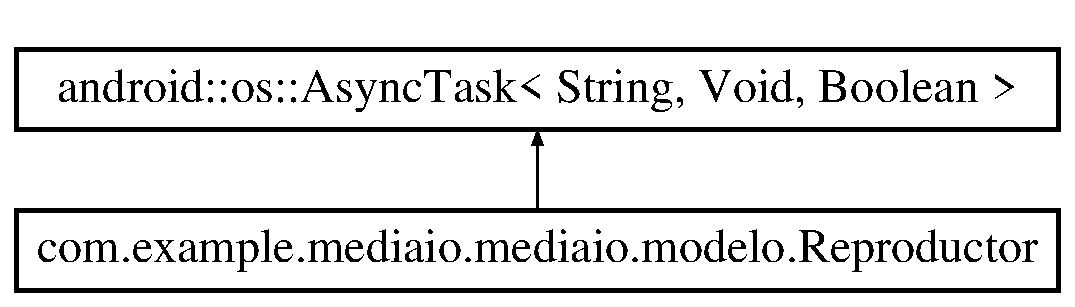
\includegraphics[height=2.000000cm]{classcom_1_1example_1_1mediaio_1_1mediaio_1_1modelo_1_1_reproductor}
\end{center}
\end{figure}
\subsection*{Métodos públicos}
\begin{DoxyCompactItemize}
\item 
\mbox{\Hypertarget{classcom_1_1example_1_1mediaio_1_1mediaio_1_1modelo_1_1_reproductor_a3bd2f8f3e81df059d21999915df3dba6}\label{classcom_1_1example_1_1mediaio_1_1mediaio_1_1modelo_1_1_reproductor_a3bd2f8f3e81df059d21999915df3dba6}} 
{\bfseries Reproductor} (Media\+Player media\+Player, String U\+RL)
\item 
\mbox{\Hypertarget{classcom_1_1example_1_1mediaio_1_1mediaio_1_1modelo_1_1_reproductor_ac08be9a63140296c37156480969bec20}\label{classcom_1_1example_1_1mediaio_1_1mediaio_1_1modelo_1_1_reproductor_ac08be9a63140296c37156480969bec20}} 
void {\bfseries pausar} ()
\item 
\mbox{\Hypertarget{classcom_1_1example_1_1mediaio_1_1mediaio_1_1modelo_1_1_reproductor_a95c5f1d9790d034b63c65afb7618df97}\label{classcom_1_1example_1_1mediaio_1_1mediaio_1_1modelo_1_1_reproductor_a95c5f1d9790d034b63c65afb7618df97}} 
void {\bfseries reproducir} ()
\end{DoxyCompactItemize}
\subsection*{Métodos protegidos}
\begin{DoxyCompactItemize}
\item 
\mbox{\Hypertarget{classcom_1_1example_1_1mediaio_1_1mediaio_1_1modelo_1_1_reproductor_abdb55b99e85a2b7a4e8e20d90f50a624}\label{classcom_1_1example_1_1mediaio_1_1mediaio_1_1modelo_1_1_reproductor_abdb55b99e85a2b7a4e8e20d90f50a624}} 
Boolean {\bfseries do\+In\+Background} (String... params)
\item 
\mbox{\Hypertarget{classcom_1_1example_1_1mediaio_1_1mediaio_1_1modelo_1_1_reproductor_a74d2e94a28189ed5bc2a699c71a29b3a}\label{classcom_1_1example_1_1mediaio_1_1mediaio_1_1modelo_1_1_reproductor_a74d2e94a28189ed5bc2a699c71a29b3a}} 
void {\bfseries on\+Post\+Execute} (Boolean result)
\end{DoxyCompactItemize}


\subsection{Descripción detallada}
Created by Marcos on 30/04/2017. 

La documentación para esta clase fue generada a partir del siguiente fichero\+:\begin{DoxyCompactItemize}
\item 
E\+:/\+Users/\+Marcos/\+Android\+Studio\+Projects/\+Media.\+io/app/src/main/java/com/example/mediaio/mediaio/modelo/Reproductor.\+java\end{DoxyCompactItemize}

\hypertarget{classcom_1_1example_1_1mediaio_1_1mediaio_1_1modelo_1_1_shared_server}{}\section{Referencia de la Clase com.\+example.\+mediaio.\+mediaio.\+modelo.\+Shared\+Server}
\label{classcom_1_1example_1_1mediaio_1_1mediaio_1_1modelo_1_1_shared_server}\index{com.\+example.\+mediaio.\+mediaio.\+modelo.\+Shared\+Server@{com.\+example.\+mediaio.\+mediaio.\+modelo.\+Shared\+Server}}
Diagrama de herencias de com.\+example.\+mediaio.\+mediaio.\+modelo.\+Shared\+Server\begin{figure}[H]
\begin{center}
\leavevmode
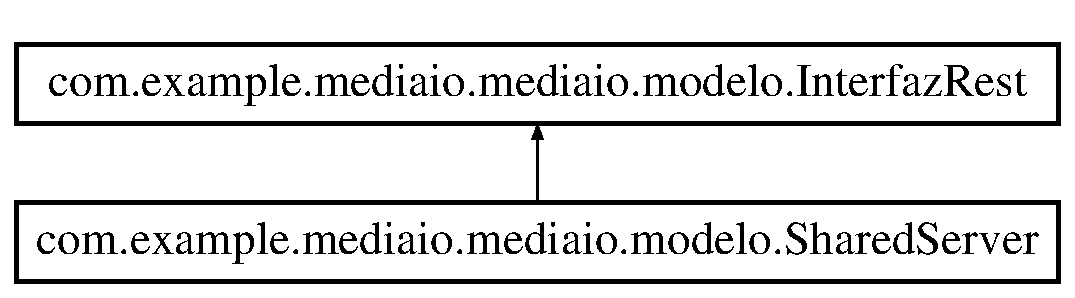
\includegraphics[height=2.000000cm]{classcom_1_1example_1_1mediaio_1_1mediaio_1_1modelo_1_1_shared_server}
\end{center}
\end{figure}
\subsection*{Métodos públicos}
\begin{DoxyCompactItemize}
\item 
\mbox{\Hypertarget{classcom_1_1example_1_1mediaio_1_1mediaio_1_1modelo_1_1_shared_server_a2c323a3b687cd93bc37169851613677e}\label{classcom_1_1example_1_1mediaio_1_1mediaio_1_1modelo_1_1_shared_server_a2c323a3b687cd93bc37169851613677e}} 
void {\bfseries existe\+Usuario\+Email} (String email, \hyperlink{classcom_1_1example_1_1mediaio_1_1mediaio_1_1modelo_1_1_j_s_o_n_callback}{J\+S\+O\+N\+Callback} callback)
\item 
\mbox{\Hypertarget{classcom_1_1example_1_1mediaio_1_1mediaio_1_1modelo_1_1_shared_server_a38f784bc140a89baeaf7786a1b468ffa}\label{classcom_1_1example_1_1mediaio_1_1mediaio_1_1modelo_1_1_shared_server_a38f784bc140a89baeaf7786a1b468ffa}} 
void {\bfseries configurar\+Token\+E\+ID} (String token, long id)
\item 
\mbox{\Hypertarget{classcom_1_1example_1_1mediaio_1_1mediaio_1_1modelo_1_1_shared_server_a40a577740aa2136f26ccd90a64910724}\label{classcom_1_1example_1_1mediaio_1_1mediaio_1_1modelo_1_1_shared_server_a40a577740aa2136f26ccd90a64910724}} 
void {\bfseries obtener\+Token} (String email, String contrasena, \hyperlink{classcom_1_1example_1_1mediaio_1_1mediaio_1_1modelo_1_1_j_s_o_n_callback}{J\+S\+O\+N\+Callback} callback)
\item 
\mbox{\Hypertarget{classcom_1_1example_1_1mediaio_1_1mediaio_1_1modelo_1_1_shared_server_af6d66c9c68d0cbc41ac6fc9199c332b8}\label{classcom_1_1example_1_1mediaio_1_1mediaio_1_1modelo_1_1_shared_server_af6d66c9c68d0cbc41ac6fc9199c332b8}} 
void {\bfseries dar\+Alta\+Usuario} (String nombre, String apellido, String email, String fecha\+Nacimiento, String contrasena, String pais, String imagen, String nombre\+Usuario, \hyperlink{classcom_1_1example_1_1mediaio_1_1mediaio_1_1modelo_1_1_j_s_o_n_callback}{J\+S\+O\+N\+Callback} callback)
\item 
\mbox{\Hypertarget{classcom_1_1example_1_1mediaio_1_1mediaio_1_1modelo_1_1_shared_server_a0c1fe1f85a8dd9ac72b9bbb1099295c4}\label{classcom_1_1example_1_1mediaio_1_1mediaio_1_1modelo_1_1_shared_server_a0c1fe1f85a8dd9ac72b9bbb1099295c4}} 
void {\bfseries Modificar\+Perfil\+Usuario} (String nombre, String apellido, String email, String fecha\+Nacimiento, String contrasena, String pais, String imagen, String nombre\+Usuario, \hyperlink{classcom_1_1example_1_1mediaio_1_1mediaio_1_1modelo_1_1_j_s_o_n_callback}{J\+S\+O\+N\+Callback} callback)
\item 
\mbox{\Hypertarget{classcom_1_1example_1_1mediaio_1_1mediaio_1_1modelo_1_1_shared_server_aacbe1fbbc2a6ebe9faa433f7ea52ea69}\label{classcom_1_1example_1_1mediaio_1_1mediaio_1_1modelo_1_1_shared_server_aacbe1fbbc2a6ebe9faa433f7ea52ea69}} 
void {\bfseries Obtener\+Canciones} (\hyperlink{classcom_1_1example_1_1mediaio_1_1mediaio_1_1modelo_1_1_j_s_o_n_callback}{J\+S\+O\+N\+Callback} callback)
\end{DoxyCompactItemize}
\subsection*{Otros miembros heredados}


\subsection{Descripción detallada}
Created by Marcos on 01/04/2017. 

La documentación para esta clase fue generada a partir del siguiente fichero\+:\begin{DoxyCompactItemize}
\item 
E\+:/\+Users/\+Marcos/\+Android\+Studio\+Projects/\+Media.\+io/app/src/main/java/com/example/mediaio/mediaio/modelo/Shared\+Server.\+java\end{DoxyCompactItemize}

\hypertarget{classcom_1_1example_1_1mediaio_1_1mediaio_1_1_login_first_activity_1_1_verificar_email}{}\section{Referencia de la Clase com.\+example.\+mediaio.\+mediaio.\+Login\+First\+Activity.\+Verificar\+Email}
\label{classcom_1_1example_1_1mediaio_1_1mediaio_1_1_login_first_activity_1_1_verificar_email}\index{com.\+example.\+mediaio.\+mediaio.\+Login\+First\+Activity.\+Verificar\+Email@{com.\+example.\+mediaio.\+mediaio.\+Login\+First\+Activity.\+Verificar\+Email}}
Diagrama de herencias de com.\+example.\+mediaio.\+mediaio.\+Login\+First\+Activity.\+Verificar\+Email\begin{figure}[H]
\begin{center}
\leavevmode
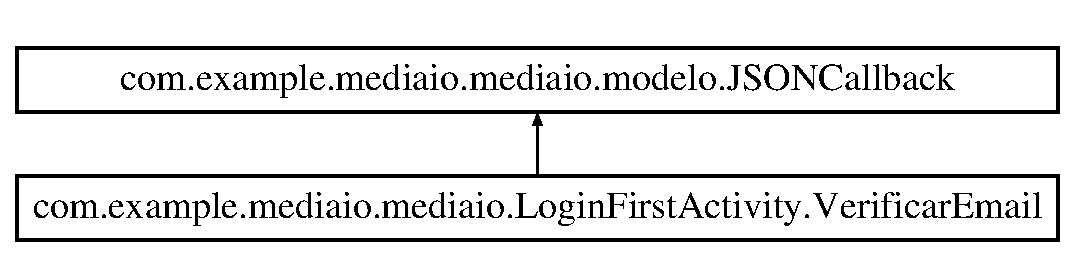
\includegraphics[height=2.000000cm]{classcom_1_1example_1_1mediaio_1_1mediaio_1_1_login_first_activity_1_1_verificar_email}
\end{center}
\end{figure}
\subsection*{Métodos públicos}
\begin{DoxyCompactItemize}
\item 
\mbox{\Hypertarget{classcom_1_1example_1_1mediaio_1_1mediaio_1_1_login_first_activity_1_1_verificar_email_ad224a450bcbbf5e30a923c5f0e7e98fc}\label{classcom_1_1example_1_1mediaio_1_1mediaio_1_1_login_first_activity_1_1_verificar_email_ad224a450bcbbf5e30a923c5f0e7e98fc}} 
void {\bfseries ejecutar} (J\+S\+O\+N\+Object json, long codigo\+Servidor)
\end{DoxyCompactItemize}


La documentación para esta clase fue generada a partir del siguiente fichero\+:\begin{DoxyCompactItemize}
\item 
E\+:/\+Users/\+Marcos/\+Android\+Studio\+Projects/\+Media.\+io/app/src/main/java/com/example/mediaio/mediaio/Login\+First\+Activity.\+java\end{DoxyCompactItemize}

%--- End generated contents ---

% Index
\backmatter
\newpage
\phantomsection
\clearemptydoublepage
\addcontentsline{toc}{chapter}{Índice}
\printindex

\end{document}
